\section{\texorpdfstring{Obvody sekvenční logiky}{Obvody sekvencni logiky}}

% =====================================================================================================================
	\begin{frame}
    \frametitle{Dělička frekvence - f/2}
		
		\begin{center}
			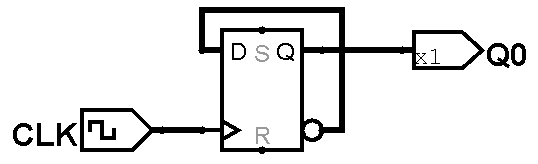
\includegraphics[scale=0.25]{fig/D_KO_divider.png}
		\end{center}
    
    \begin{center}
			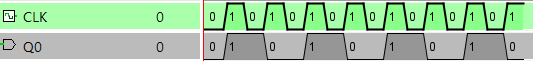
\includegraphics[scale=0.5]{fig/D_KO_divider_diag.png}
		\end{center}
	
		\begin{itemize}
			\item Výsledná frekvence je poloviční, protože je jen jedna náběžná hrana na periodu hodin.
      \item Společně se signálem hodin vytváří čítač 3 až 0.
      \item Je základním stavebním kamenem asynchronního čítače.
		\end{itemize}
	
	\end{frame}
  
% =====================================================================================================================
	\begin{frame}
    \frametitle{Asynchronní čítač dolů}
		
		\begin{center}
			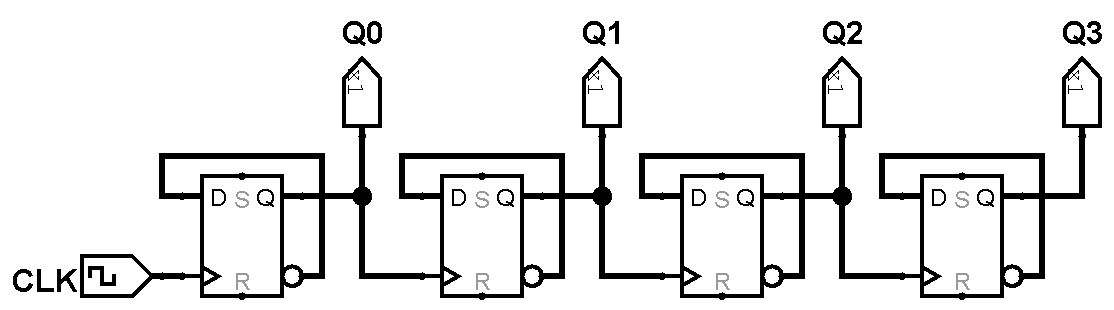
\includegraphics[scale=0.25]{fig/D_KO_cnt_down.png}
		\end{center}
    
    \begin{center}
			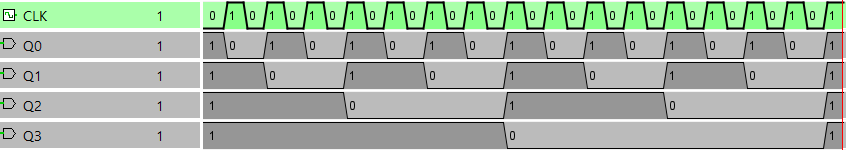
\includegraphics[scale=0.5]{fig/D_KO_cnt_down_diag.png}
		\end{center}
	
		\begin{itemize}
			\item vstupy a výstupy nabývají pouze logických hodnot, tj. 0 1,
			\item stav výstupu závisí navíc na časové posloupnosti (sekvenci) vstupů,
			\item obvod obsahuje paměť pro uchování stavu.

		\end{itemize}
	
	\end{frame}
  
% =====================================================================================================================
	\begin{frame}
    \frametitle{Asynchronní čítač nahoru}
		
		\begin{center}
			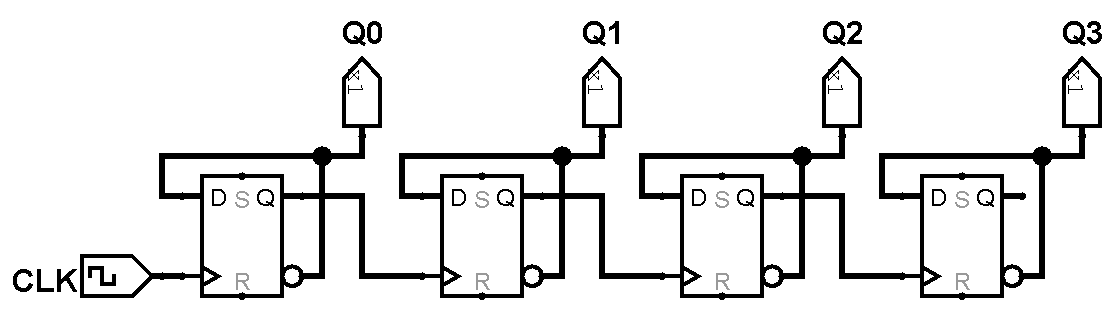
\includegraphics[scale=0.25]{fig/D_KO_cnt_up.png}
		\end{center}
    
    \begin{center}
			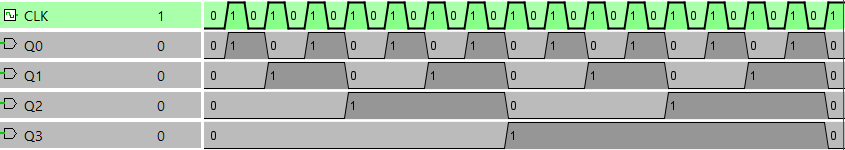
\includegraphics[scale=0.5]{fig/D_KO_cnt_up_diag.png}
		\end{center}
	
		\begin{itemize}
			\item vstupy a výstupy nabývají pouze logických hodnot, tj. 0 1,
			\item stav výstupu závisí navíc na časové posloupnosti (sekvenci) vstupů,
			\item obvod obsahuje paměť pro uchování stavu.

		\end{itemize}
	
	\end{frame}
  
% =====================================================================================================================
	\begin{frame}
    \frametitle{Posuvný registr}
		
		\begin{center}
			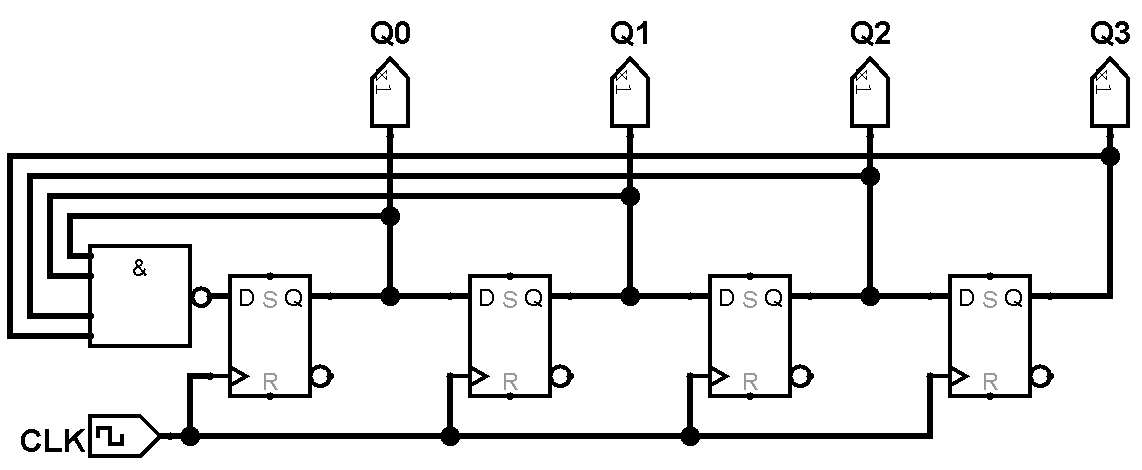
\includegraphics[scale=0.25]{fig/D_KO_shift.png}
		\end{center}
    
    \begin{center}
			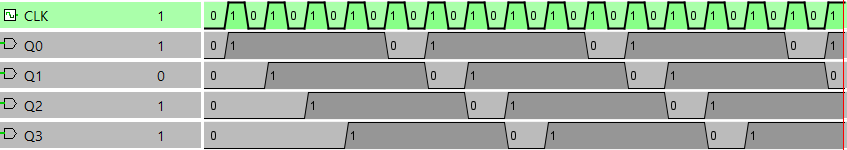
\includegraphics[scale=0.5]{fig/D_KO_shift_diag.png}
		\end{center}
	
		\begin{itemize}
			\item vstupy a výstupy nabývají pouze logických hodnot, tj. 0 1,
			\item stav výstupu závisí navíc na časové posloupnosti (sekvenci) vstupů,
		\end{itemize}
	
	\end{frame}
  
% =====================================================================================================================
	\begin{frame}
    \frametitle{Synchronní čítač - návrh pro 3 bity}
		
		\begin{minipage}[t][\textheight][t]{0.45\textwidth}
    \vspace{10mm}
    
    \begin{itemize}
      \item Synchronní - společné hodiny všem D-KO,
      \item přechod mezi stavy musí být stanoven kombinační logikou,
      \item proměnné:
      
      \begin{itemize}
        \item[$Q$] ... aktuální stav,
        \item[$D$] ... budoucí stav,
        \item[$Y$] ... $Y=Q \Rightarrow$ Moore,
      \end{itemize}
    \end{itemize}
    
		\end{minipage}
		\begin{minipage}[t][\textheight][t]{0.5\textwidth}
		\vspace{10mm}
		\begin{center}
			\begin{tabular}{ c c c | c c c }
				$Q2$ & $Q1$ & $Q0$ & $D2$ & $D1$ & $D0$\\
				\hline
				0 & 0 & 0 & 0 & 0 & 1 \\
				0 & 0 & 1 & 0 & 1 & 0 \\
				0 & 1 & 0 & 0 & 1 & 1 \\
				0 & 1 & 1 & 1 & 0 & 0 \\
        1 & 0 & 0 & 1 & 0 & 1 \\
				1 & 0 & 1 & 1 & 1 & 0 \\
				1 & 1 & 0 & 1 & 1 & 1 \\
				1 & 1 & 1 & 0 & 0 & 0 \\
			\end{tabular}
		\end{center}

		\end{minipage}
		
	\end{frame}
  
% =====================================================================================================================
	\begin{frame}
    \frametitle{Synchronní čítač - KM pro D0}
    \begin{center}
      \begin{karnaugh-map}[4][2][1][$Q0$][$Q1$][$Q2$]
        \minterms{0,2,4,6}
        \implicantedge{0}{4}{2}{6}
        % ====== vlastní čáry ======

        % A = 1 (druhý řádek)
        \draw[very thick] (-0.15,1) -- (-0.15,0);

        % B = 1 (sloupce 3 a 4)
        \draw[very thick] (2,2.3) -- (4,2.3);

        % C = 1 (sloupce 2 a 3)
        \draw[very thick] (1,2.15) -- (3,2.15);

      \end{karnaugh-map}
    \end{center}
    
    
    \begin{itemize}
      \item $D0 = \textcolor{red}{\bar{Q0}}$
      \item Stejná negace jako u děličky frekvence. 
    \end{itemize}
		
	\end{frame}

% =====================================================================================================================
	\begin{frame}
    \frametitle{Synchronní čítač - KM pro D1}
    
    \begin{center}
      \begin{karnaugh-map}[4][2][1][$Q0$][$Q1$][$Q2$]
        \minterms{1,2,5,6}
        \implicant{1}{5}
        \implicant{2}{6}
        
        % ====== vlastní čáry ======

        % A = 1 (druhý řádek)
        \draw[very thick] (-0.15,1) -- (-0.15,0);

        % B = 1 (sloupce 3 a 4)
        \draw[very thick] (2,2.3) -- (4,2.3);

        % C = 1 (sloupce 2 a 3)
        \draw[very thick] (1,2.15) -- (3,2.15);

      \end{karnaugh-map}
    \end{center}
		
    \begin{itemize}
      \item $D0 = \textcolor{red}{Q0\bar{Q1}} + \textcolor{green}{\bar{Q0}Q1}$
      \item Odpovídá funkci XOR. 
    \end{itemize}
    
	\end{frame}
  
% =====================================================================================================================
	\begin{frame}
    \frametitle{Synchronní čítač - KM pro D2}
    
    \begin{center}
      \begin{karnaugh-map}[4][2][1][$Q0$][$Q1$][$Q2$]
        \minterms{3,4,5,6}
        \implicant{3}{3}
        \implicantedge{4}{4}{6}{6}
        \implicant{4}{5}
        
        % ====== vlastní čáry ======

        % A = 1 (druhý řádek)
        \draw[very thick] (-0.15,1) -- (-0.15,0);

        % B = 1 (sloupce 3 a 4)
        \draw[very thick] (2,2.3) -- (4,2.3);

        % C = 1 (sloupce 2 a 3)
        \draw[very thick] (1,2.15) -- (3,2.15);

      \end{karnaugh-map}
    \end{center}
		
    \begin{itemize}
      \item $D0 = \textcolor{red}{Q0Q1\bar{Q2}} + \textcolor{green}{\bar{Q0}Q2} + \textcolor{orange}{\bar{Q1}Q2} = Q0Q1\bar{Q2} + \overline{Q0Q1}Q2$
      \item Odpovídá funkci AND a XOR. 
    \end{itemize}
    
	\end{frame}
  
% =====================================================================================================================
	\begin{frame}
    \frametitle{Synchronní čítač - zapojení}
		
		\begin{center}
			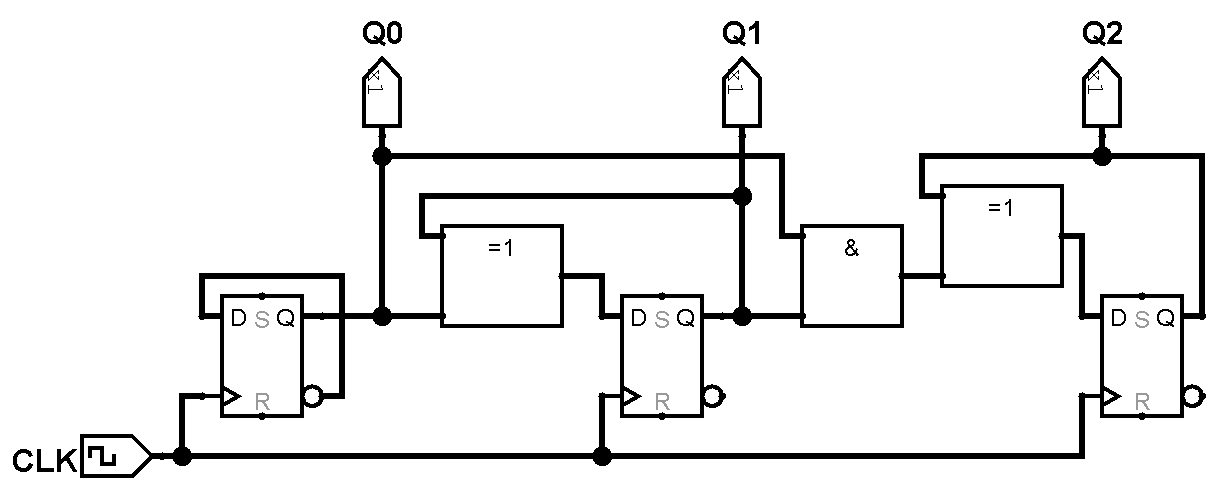
\includegraphics[scale=0.25]{fig/D_KO_cnt_sync.png}
		\end{center}
    
    \begin{center}
			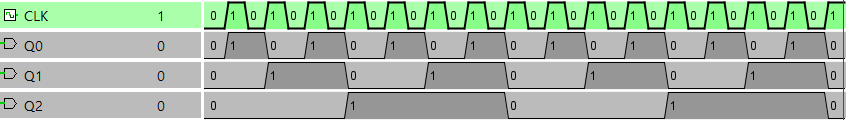
\includegraphics[scale=0.5]{fig/D_KO_cnt_sync_diag.png}
		\end{center}
	
	
	\end{frame}